% Explain the genral stucture of the debugger
The debugger \acrfull{erd} is implemented using the debugging library \emph{rust-debug}.
That library provides all of the needed functionalities for retrieving debug information from the \gls{DWARF} format.
The debugger also uses the \emph{probe-rs} library for controlling the \gls{mcu}.
It is also used for accessing the registers and memory of the \gls{mcu}.


The debugger is made up of three modules, the first one is called \acrshort{cli}.
Its main functionality is to handle the input from the console and the output to it.
The second module is called DebugAdapter.
It also handles the input and output, but in the form of \gls{dap} messages.
This module is for supporting \glspl{gui} that use the \gls{dap} protocol to display debug information.
The last module is called Debugger, and it runs in a separate thread from the other two modules.
This is the module that uses the \emph{rust-debug} and \emph{probe-rs} library to get debug information.
It is also used to control the debug target.
Figure \ref{fig:ERDStruct} shows a diagram of how these modules are structured.
Also all of the code for \gls{erd} can be found in this git repository \cite{erd}.


\begin{figure}[h]
	\centering
	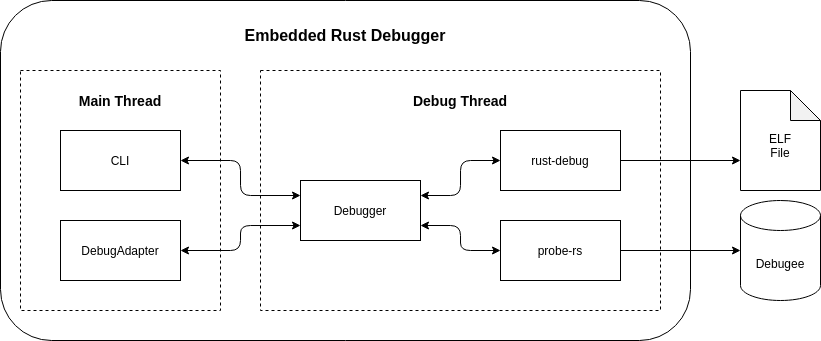
\includegraphics[width=1.0\textwidth]{debugger_structure.png}
	\caption{Diagram showing the structure of ERD.}
	\label{fig:ERDStruct}
\end{figure}


\subsubsection{The CLI module}
\subimport{}{cli.tex}


\subsubsection{The Debug Adapter module}
\subimport{}{debug_adapter.tex}


\subsubsection{The Debugger Module}
The debugger module is designed as a server that listens for commands through a channel.
It is running in a separate thread from the \acrshort{cli} and the debug adapter, which is called the debug thread.
There is two states in which the debug thread can be in, that is in the attached or detached state.
The two states are different in that the attached state can access the debug target and the \gls{DWARF} file.


The debug thread is started by the main thread and starts in the detached state.
In the detached state only the configuration and exit commands work.
The other commands requires that the debug target is attached.
But if one of those commands is received then the debug thread will try to enter the attached state.
This can only happen if all the required configuration are set.
If one of the configuration are missing then an error will be sent as a response.


When the debug thread is in the attached state it can use the \emph{rust-debug} library to retrieve debug information.
It can also use the \emph{probe-rs} library for controlling the debug target and reading the registers and memory.
The relation between the libraries can be seen in figure \ref{fig:debugger}.


\begin{figure}[h]
	\centering
	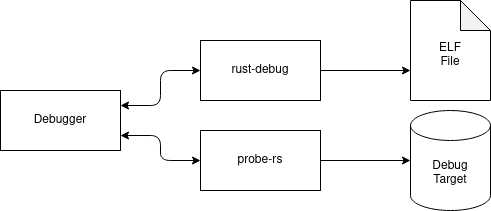
\includegraphics[width=1.0\textwidth]{debugger.png}
	\caption{A diagram showing the relations between the debugger, the \emph{ELF} file, the debug target and the two libraries \emph{rust-debug} and \emph{probe-rs}.}
	\label{fig:debugger}
\end{figure}


\subsubsubsection{Retrieving Debug Information}
The debugger module retrieves debug information by using the \emph{rust-debug} library.
This library sometimes requires a data structure that contain the values of some registers and memory addresses.
Those function will return an enum that tells if a value is needed and where that value is located.
Thus the debugger module will use the \emph{probe-rs} library to read the needed value, which is then added to the data structure.
This repeats until no more values are needed, and the result of the evaluation can be retrieved.
The values in the data structure are removed every time the debug target starts executing again.
This is such that no old values are used, and it works because the debug target must be stopped to use related commands.



\subsubsubsection{Simultaneous Handling of Requests And Events}
% How the debugger handles request and events simultaneously.
The debug thread polls the channel for incoming request and the state of the debug target.
This enables the debug thread to simultaneously handle requests from the user, and events from the debug target.
There is a boolean that keeps track if the debug target is running.
It is used to stop the pulling of the targets state when the debug target is stopped.
This is done because the debug target cannot start executing on its own.


\subsubsubsection{Optimization of Repeated Variable Evaluation}
% How it handles request for stackframes and variables.
To improve on the performance of the debugger it will temporarily store the values of the stack trace.
This allows for fast repetitive lookup of information present in the stack trace.
The stored stack trace is removed any time the debug target starts executing again.
This ensures that it always gives the correct values and not the old ones.


Note that if a request is received to evaluate one variable, the debugger will then perform a stack trace instead, or read from the temporarily stored stack trace.
This simplifies the implementation a lot and also makes the subsequent evaluation requests faster.

